A helpdesk alkalmazás \aref{ch:uzleti_igenyek}. fejezetben leírtaknak megfelelően szolgál ki három különböző e-mail címet:

\begin{itemize}
	\item a \texttt{generic} sorhoz tarozó  \href{mailto:helpdesk.gdf@yandex.com}{\nolinkurl{helpdesk.gdf@yandex.com}}-ot, 
	\item a \texttt{travel} sorhoz tarozó  \href{mailto:helpdesk.gdf.travel@yandex.com}{\nolinkurl{helpdesk.gdf.travel@yandex.com}}-ot,
	\item és a \texttt{theater} sorhoz tarozó  \href{mailto:h.gdf.theater@gmx.com}{\nolinkurl{h.gdf.theater@gmx.com}}-ot.
\end{itemize}



\section{Alkalmazás elindítása}\label{sec:elinditas}
Az alkalmazás a \texttt{start.sh} bash \texttt{script}tel indítható el. A \texttt{script} két dolgot csinál:
\begin{enumerate}
	\item a \texttt{docker-compose} parancssal elindítja a docker \emph{container}eket~(\ref{sec:docker} pont),
	\item  \texttt{helpdesk} domain névvel hozzáadja az Nginx (\ref{sec:nginx} pont) IP címét a \mbox{\texttt{/etc/hosts}} állományhoz.
\end{enumerate}

A \texttt{script} indítása után a helpdesk alkalmazás elérhető a \href{http://helpdesk}{http://helpdesk} domain alatt.

\section{Virtuális gép}
Annak érdekében, hogy a létrehozott alkalmazást könnyedén ki lehessen próbálni, egy virtuális számítógépre letöltöttem az alkalmazás $1.0.0$ verzióját. A virtuális számítógép elérhető a DVD mellékleten, vagy letölthető a: \\
\href{http://todo}{todo} címről.

A virtuális gépbe a \texttt{dxqrpj} felhasználóval és jelszóval lehet bejelentkezni. Bejelentkezés után a háttérben automatikusan elindul a helpdesk alkalmazás, így \aref{sec:elinditas} pontban írt \texttt{start.sh} bash \texttt{script} kézi futtatása nem szükséges.

Az első indítás a virtuális számítógép szűk erőforrásai, valamint a \emph{docker image}-ek letöltése miatt, --~a natív indítástól eltérő módon~-- akár 5-10 percet is igénybe vehet.

A helpdesk alkalmazás elindulása után, a Firefox webböngészővel elérhető a \href{http://helpdesk}{http://helpdesk} cím. A böngésző három felhasználót tárol:
\begin{description}
	\item[admin] felhasználót, aki az \texttt{admin\textunderscore user} jogkörrel (\ref{sec:Jogosultságkezelés} pont) rendelkezik, és a \texttt{generic} sorhoz tartozik;
	\item[test] felhasználót, aki a \texttt{regular\textunderscore user} jogkörrel (\ref{sec:Jogosultságkezelés} pont) rendelkezik, és a \texttt{generic} sorhoz tartozik.;
	\item[testTheater] felhasználót, aki szintén a \texttt{regular\textunderscore user} jogkörrel rendelkezik, viszont a \texttt{theater} sorhoz tartozik.
\end{description}
 
A felhasználók bejelentkezése után elérhetőek \aref{todo} pontban összegyűjtött funkciók. Az alkalmazás a már említett három --~\texttt{generic}, \texttt{travel} és \texttt{theater}~-- sorhoz tartozó e-mail címről fogad és küld üzeneteket. Az indítás után nem sokkal, az alkalmazásban megjelennek az e-mail címekre küldött teszt üzenetek.



\section{Deployment}
A könyebb bemutathatóság érdekében a szemléletesebb szolgáltatásokat --~hogy ne a docker daemon által kiosztott IP címen keresztül kelljen elérni~--   a docker hálózaton kívül is elérhetővé tettem. 

A \texttt{docker-compose} (\ref{sec:elinditas}) által elindított \emph{container}eket \aref{fig:deployment_diagram}. ábrán foglaltam össze. Az ábrán feltüntettem, hogy az adott \emph{container}t a \texttt{localhost} melyik portján lehet elérni.


\begin{figure}[hbt] 
	\centering
	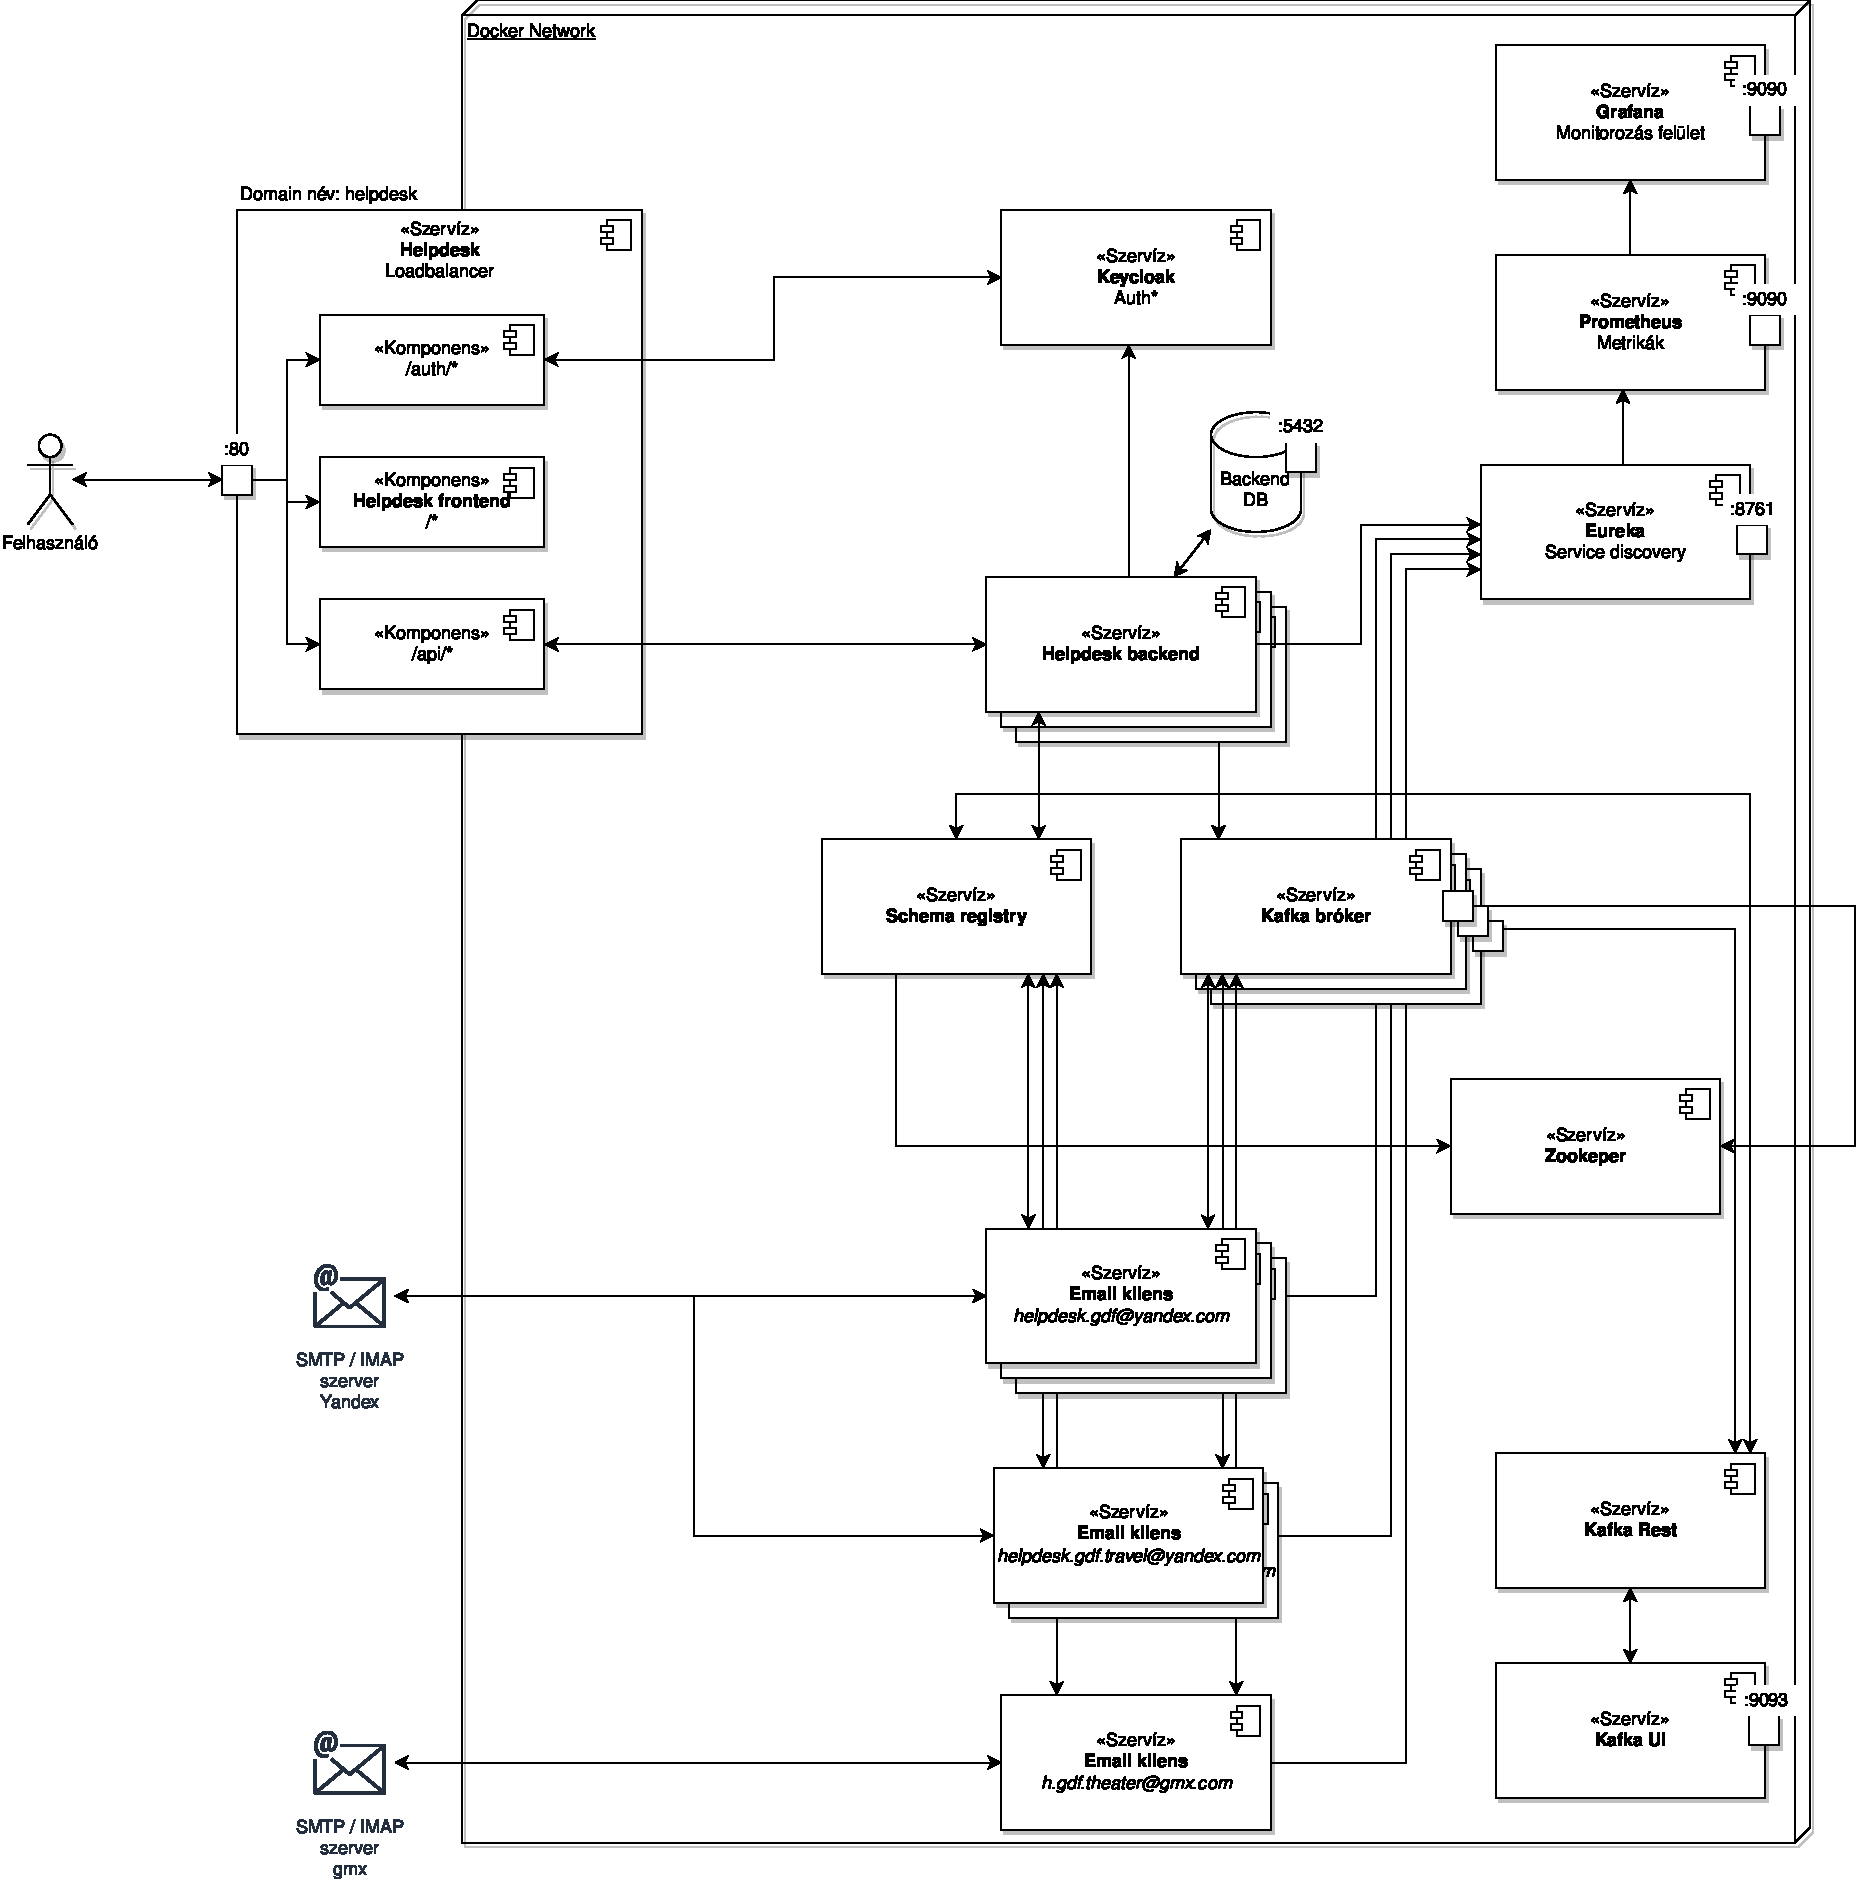
\includegraphics[width=0.95\textwidth]{deployment_diagram_drawio.pdf}
	\caption[Deployment diagram]{Deployment diagram}
	\label{fig:deployment_diagram}
	\floatfoot{Forrás: saját ábra}
\end{figure}



\section{Több példány}
A különböző szolgáltatásokból a terhelésnek megfelelően eltérő számú példány indul el:

\begin{itemize}
	\item a helpdesk-backendből három,
	\item a \texttt{theater} sort kezelő email-kliensből egy,
	\item a \texttt{travel} sort kezelő email-kliensből kettő,
	\item a \texttt{generic} sort kezelő email-kliensből három,
	\item és a Kafka brókerből (\ref{sec:kafka_topics}) szintén három darab.
\end{itemize}

A példányok metrikáit (\ref{sec:metrikak} pont) nyomon lehet követni az erre a célra létrehozott Grafana oldalon (\ref{fig:backend_receive_kafka} ábra). Az oldal elérhető a  \texttt{Spring metrics} menüpont alatt.

\Aref{fig:backend_receive_kafka} ábrán csak a Grafana oldal legfelső néhány panele látható, az instance-okra lebontott legfontosabb mérőszámokkal:

\begin{itemize}
	\item a legfelső sorban a Java Virtual Machine, által aktuálisan felhasznált Heap space,	
	\item alatta a feldolgozott Kafka üzenetek száma,
	\item a harmadik sorban a Trace log bejegyzések száma,
	\item míg az utolsó sorban az aktuális REST lekérések száma látható.
\end{itemize}



\section{E-mail fogadásának és küldésének folyamata}
\Aref{ch:felepites}. fejezetben \aref{fig:path_of_an_email}. ábrán bemutattam egy e-mail fogadásának elméleti útját. Most \aref{fig:email_send_receive_visible}. ábrán bemutatom hogyan követhető végig a rendszerben egy e-mail valódi útja.

E-mail fogadása:
\begin{enumerate}
	\item Egy teszt üzenet érkezik a \href{mailto:helpdesk.gdf.travel@yandex.com}{\nolinkurl{helpdesk.gdf.travel@yandex.com}} címre
	\emph{E-mail fogadásának és küldésének folyamata} tárggyal.
	\item Az e-mail kliens kafka üzenetként publikálja az üzenetet az \texttt{email.in.v1.pub} topicba (\ref{fig:email_client_send_kafka}. ábra).
	\item A backend megkapja a kafka üzenetet (\ref{fig:backend_receive_kafka}. ábra).
	\item A backend elmenti az új üzenet az adatbázisba (\ref{fig:datbase_received_email}. ábra).
	\item A felhasználói felületen (\ref{fig:frontend_read_email}. ábra) elérhető az új üzenet.
\end{enumerate}

\bigskip

E-mail küldése:
\begin{enumerate}
	\item A felhasználó elküldi a válaszát a felhasználói felületen (\ref{fig:frontend_send_answer}. ábra).
	\item A backend megkapja az üzenetet és eltárolja az adatbázisba (\ref{fig:database_answer}. ábra).
	\item A \texttt{h.gdf.theater\textunderscore gmx.com.v1.pub} topicban megjelenik. (\ref{fig:kafka_topic_send_email}. ábra) a backend által publikált kafka üzenet.
	\item A topicra feliratkozott e-mail kliens fogadja és továbbítja az üzenetet. (\ref{fig:email_client_receives_kafka}. ábra).
\end{enumerate}
 

\begin{figure}
	\begin{subfigure}{.49\textwidth}
		\centering
		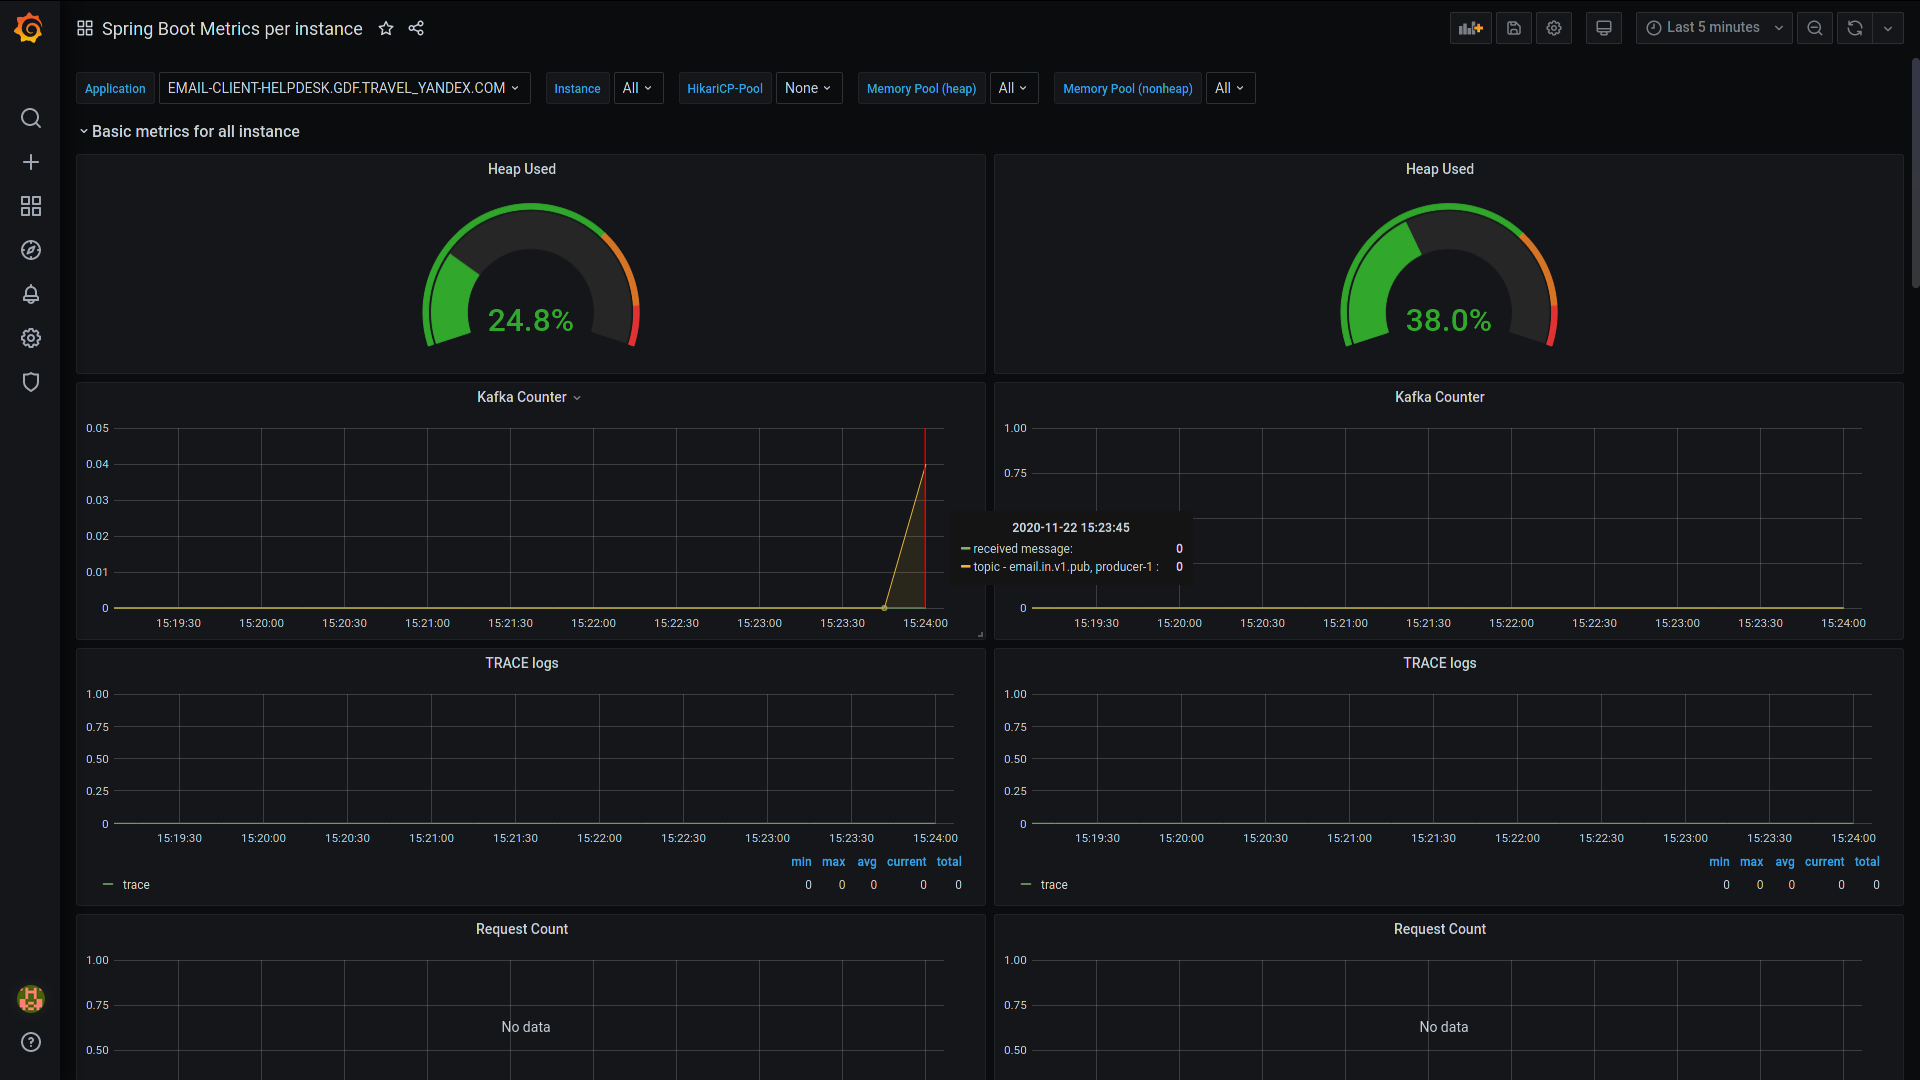
\includegraphics[width=.9\linewidth]{email_client_sending_kafka_message.png}  
		\caption{Az egyes instance kafka üzenet küld}
		\label{fig:email_client_send_kafka}
	\end{subfigure}
	\begin{subfigure}{.49\textwidth}
		\centering
		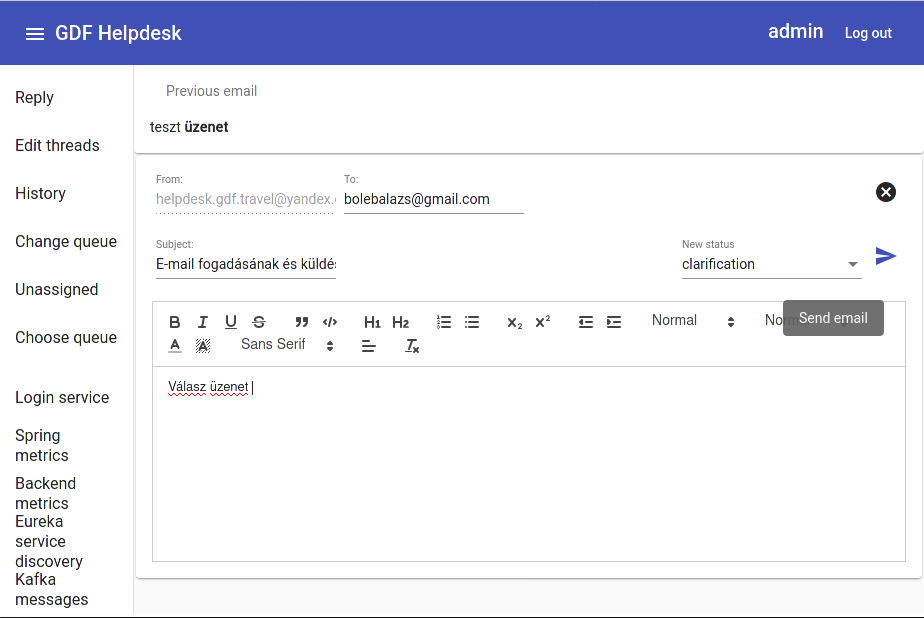
\includegraphics[width=.9\linewidth]{helpdesk_frontend_send_email.png}  
		\caption{A felületen válasz e-mailt küld a felhasználó}
		\label{fig:frontend_send_answer}
	\end{subfigure}
	
	\quad
	
	\begin{subfigure}{.49\textwidth}
		\centering
		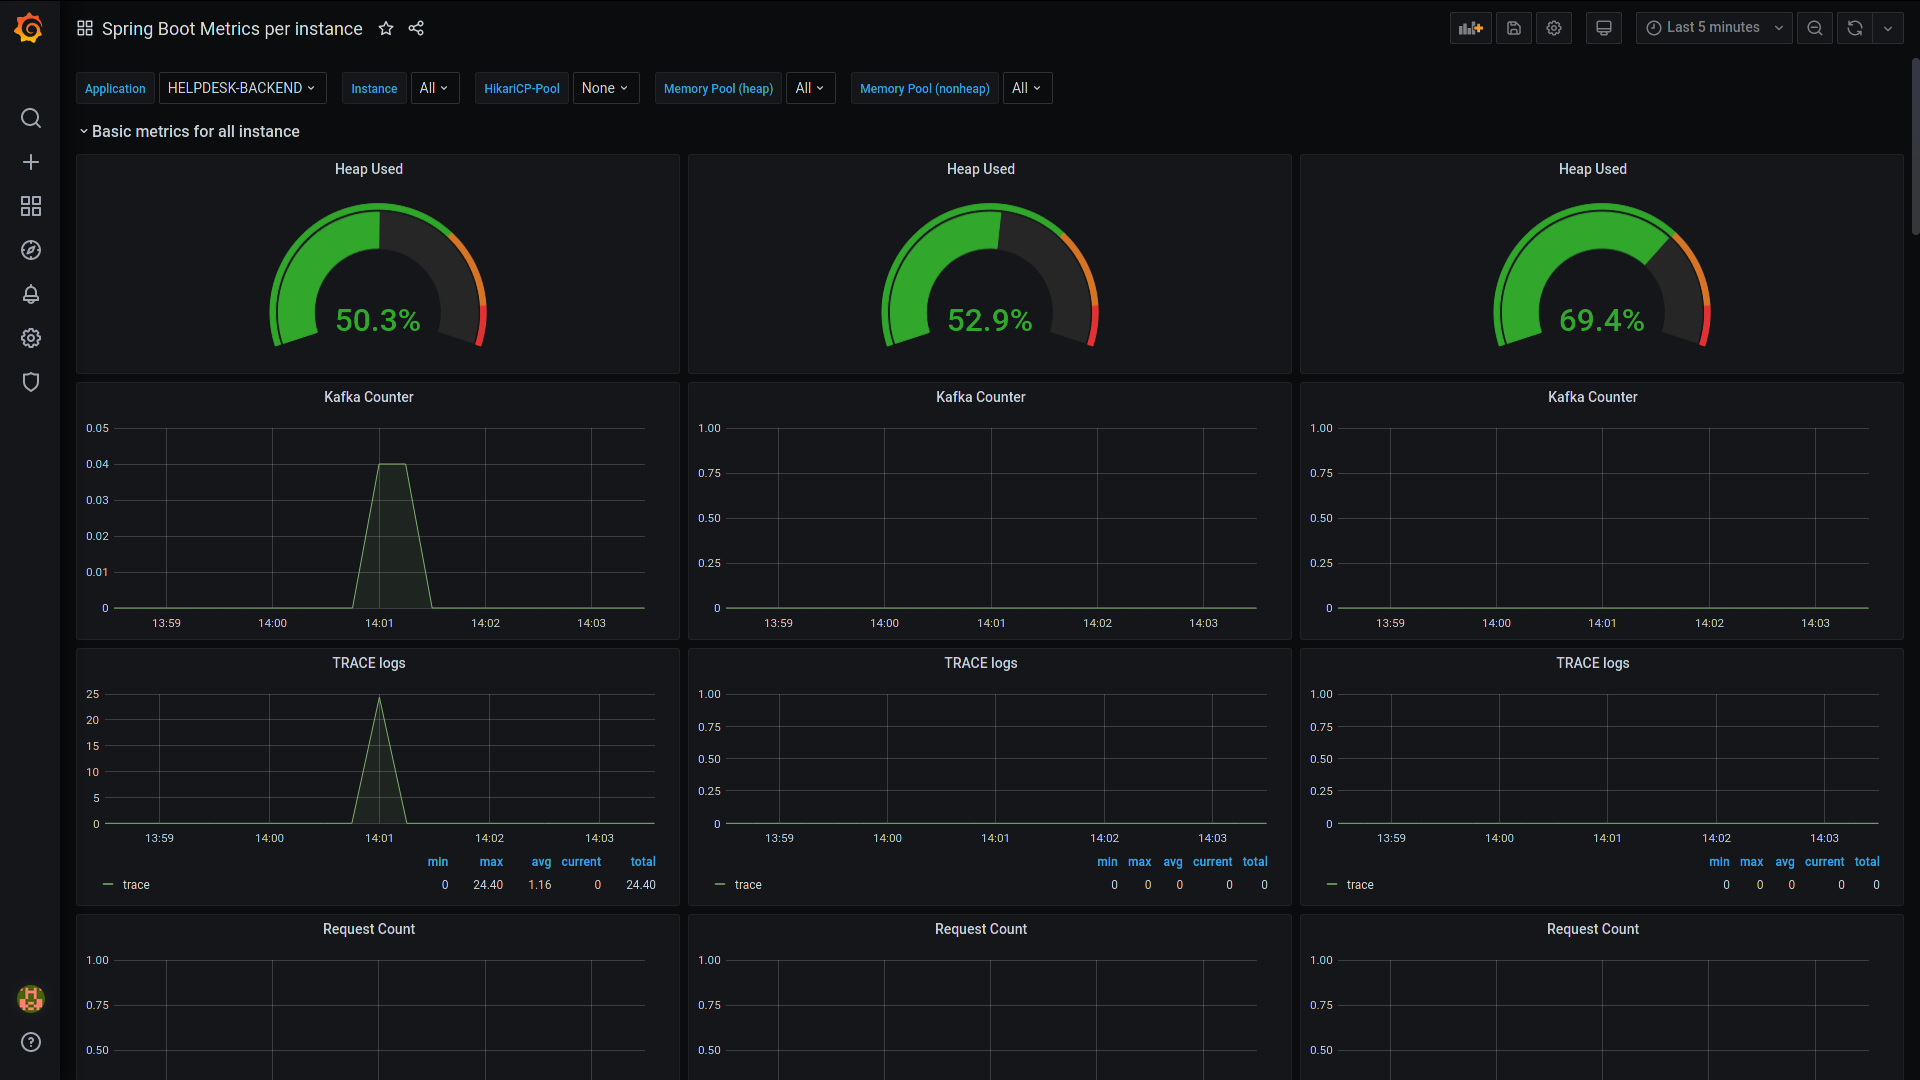
\includegraphics[width=.9\linewidth]{backend_receiving_email_from_kafka.png}  
		\caption{Az egyes instance kafka üzenet fogad}
		\label{fig:backend_receive_kafka}
	\end{subfigure}
	\begin{subfigure}{.49\textwidth}
		\centering
		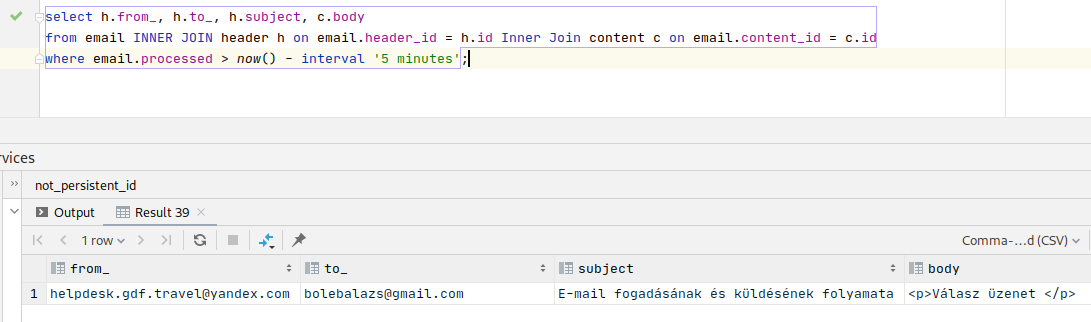
\includegraphics[width=.9\linewidth]{database_with_the_answer.png}  
		\caption{A válasz e-mail az adatbázisban}
		\label{fig:database_answer}
	\end{subfigure}

	\quad

\begin{subfigure}{.49\textwidth}
	\centering
	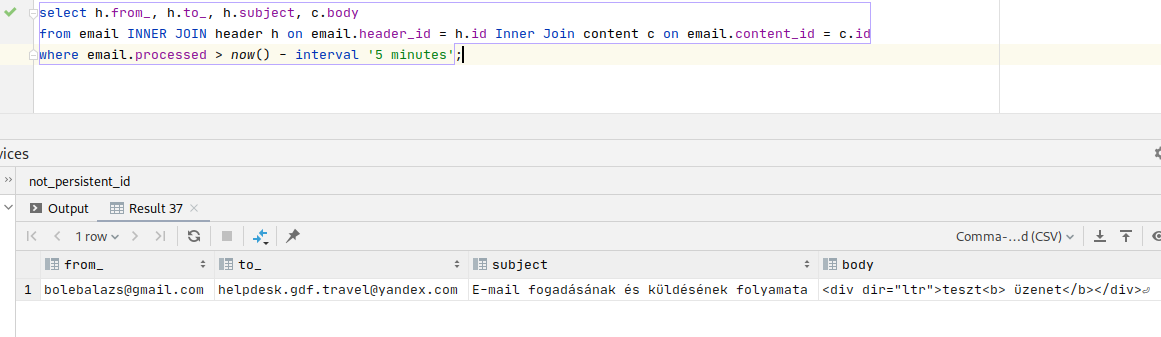
\includegraphics[width=.9\linewidth]{databse_incoming_email.png}  
	\caption{Az új e-mail az adatbázisban}
	\label{fig:datbase_received_email}
\end{subfigure}
\begin{subfigure}{.49\textwidth}
	\centering
	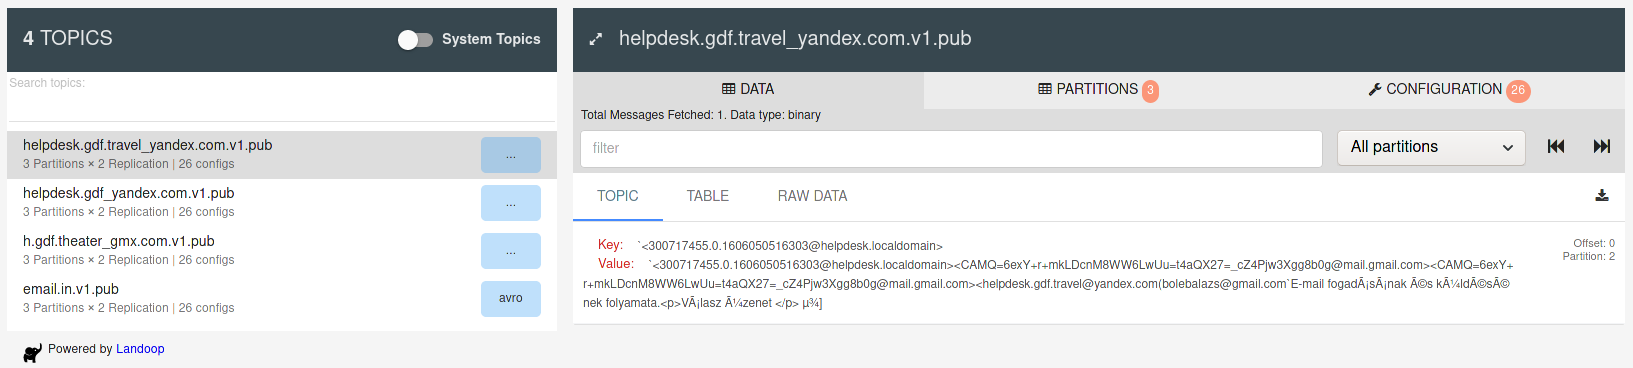
\includegraphics[width=.9\linewidth]{kafka_topic_with_the_sent_email.png}  
	\caption{A \texttt{h.gdf.theater\textunderscore gmx.com.v1.pub} topic új üzenete}
	\label{fig:kafka_topic_send_email}
\end{subfigure}

	\quad

\begin{subfigure}{.45\textwidth}
	\centering
	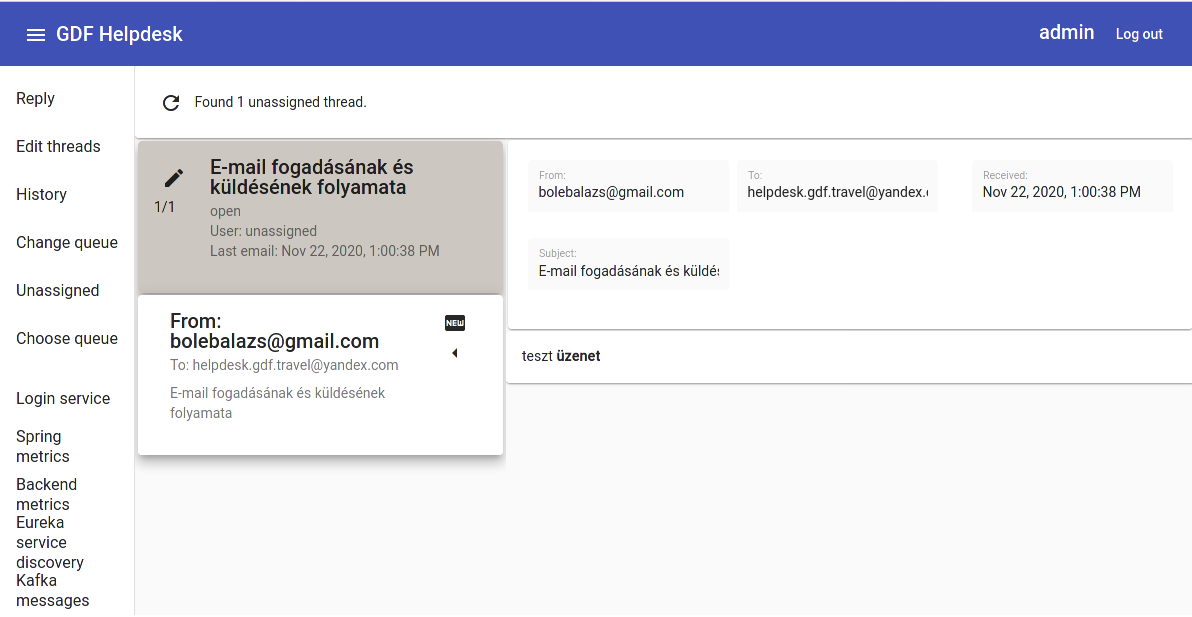
\includegraphics[width=.9\linewidth]{helpdesk_frontend_receive_incoming_email.png}  
	\caption{A felületen elérhető az új e-mail}
	\label{fig:frontend_read_email}
\end{subfigure}
\begin{subfigure}{.45\textwidth}
	\centering
	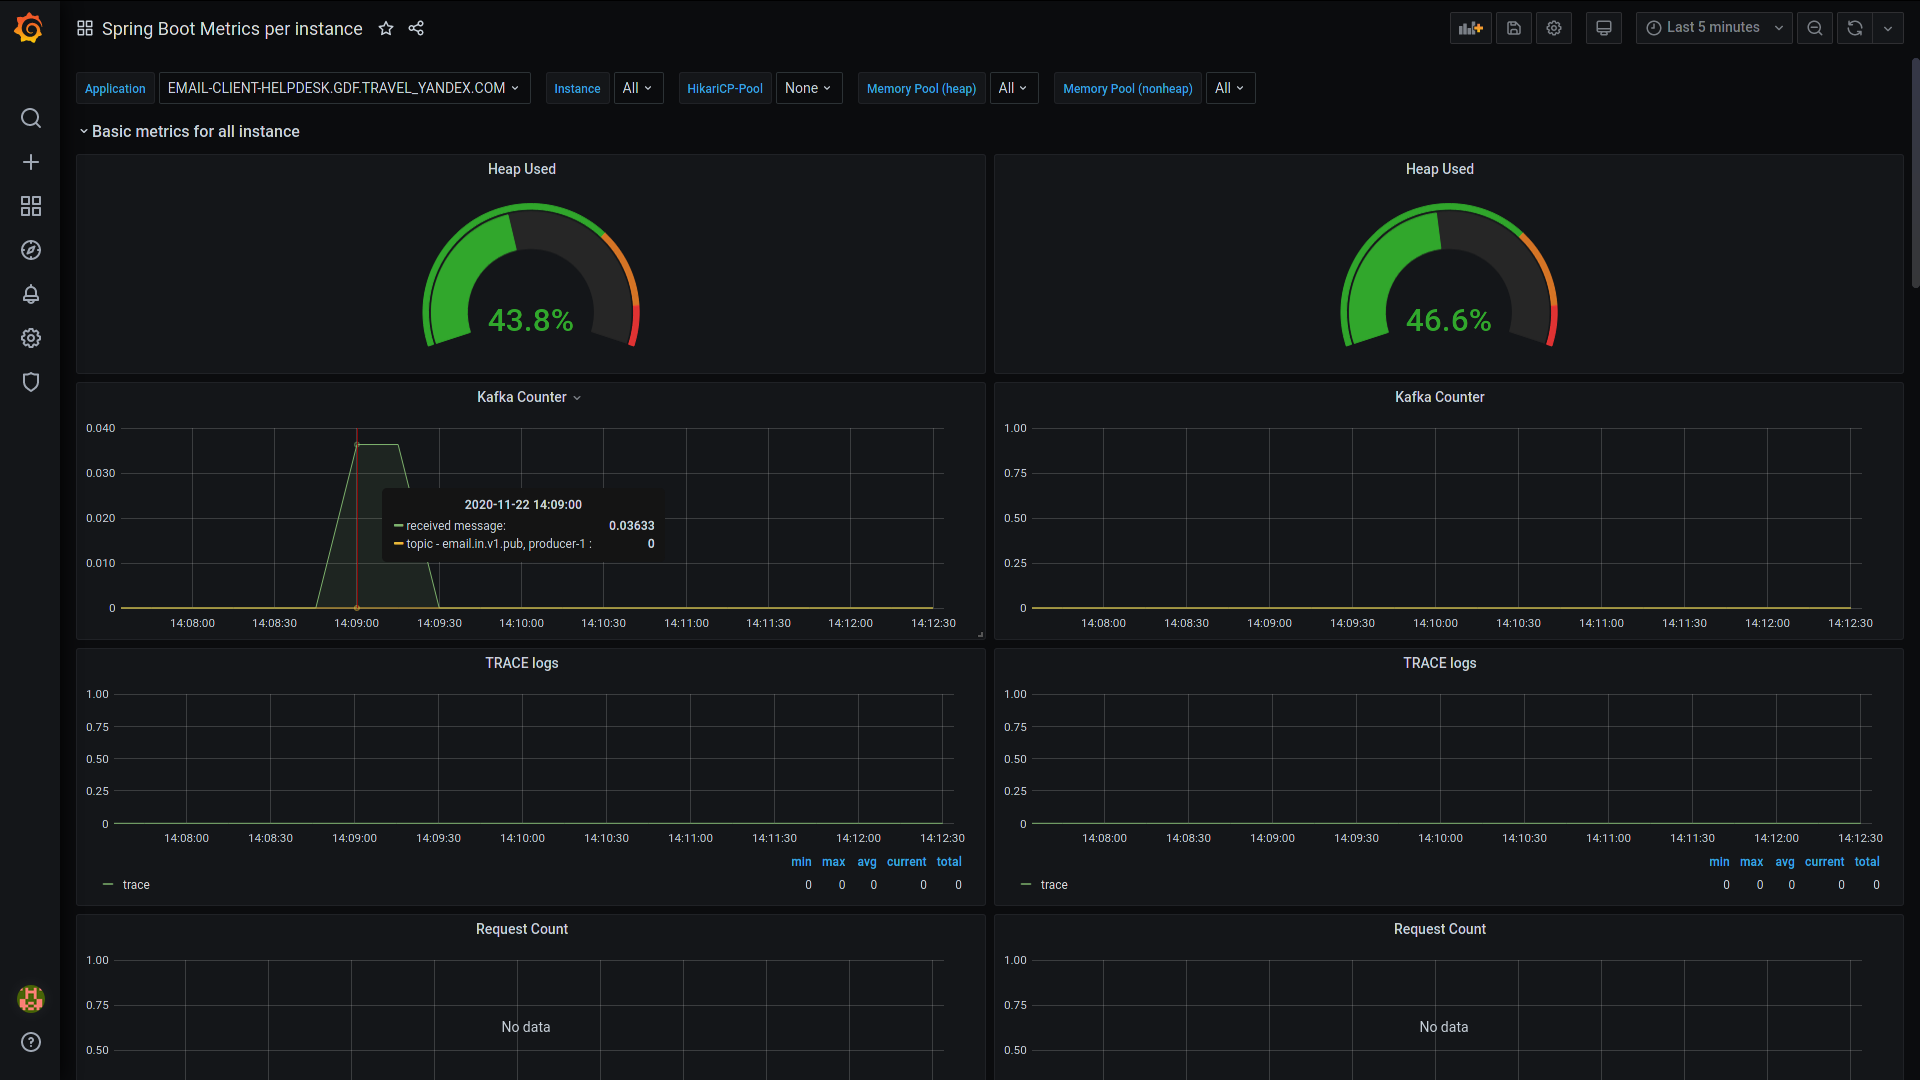
\includegraphics[width=.9\linewidth]{email_client_sending_email.png}  
	\caption{Az egyes instance kafka üzenet fogad}
	\label{fig:email_client_receives_kafka}
\end{subfigure}

	\caption[E-mail fogadásának és küldésének folyamata]{E-mail fogadásának és küldésének folyamata során követhető lépések}
	\label{fig:email_send_receive_visible}
\end{figure}



\section{Adatbázistáblák}
A helpdesk backend adatbázistábláit \aref{fig:extended_database_uml}. ábra tartalmazza.

\begin{figure}[hbt] 
	\centering
	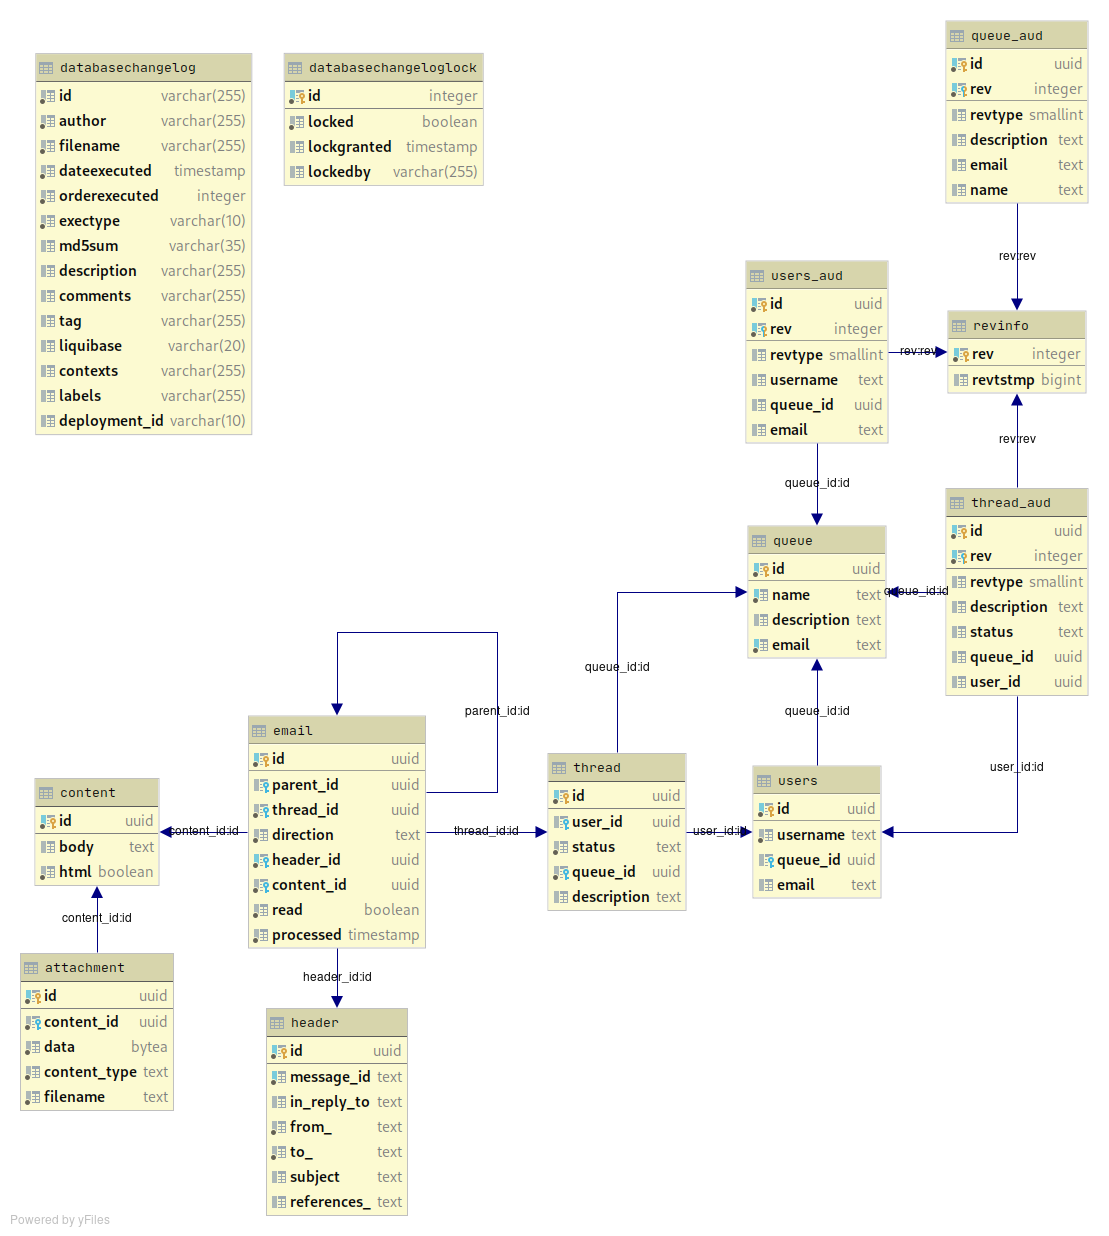
\includegraphics[width=0.85\textwidth]{extended_database_uml.png}
	\caption{A backend összes adatbázistáblája}
	\label{fig:extended_database_uml}
	\floatfoot{Forrás: saját ábra}
\end{figure}


\subsection{Liquibase}\label{sec:liquibase}
A \texttt{databasechangelog} és \texttt{databasechangeloglock} táblákat a Liquibase (\ref{sec:adatbazis}. pont) az adatbázis séma verziójának karbantartására használja:
\begin{description}
	\item[databasechangelog] tábla tartalmazza a \mbox{\texttt{resources/db.changelog}} könyvtárban található,  \mbox{\texttt{db.changelog-master.yaml}} állományban tárolt utasítások futási eredményeit.
	
	\item[databasechangeloglockot] minden végrehajtásnál a Liquibase példánya  zárolja, ezzel biztosítva hogy mindig maximum egy példány hajtson végre módosításokat az adatbázison (lásd \ref{sec:konkurencia_kezekese} pont, pesszimista konkurenciakezelési stratégia).
\end{description}

A helpdesk backend szolgáltatás minden induláskor elindítja a Liquibase-t. A Liquibase csatlakozik az adatbázishoz a \texttt{helpdesk} felhasználóval, és lefuttatja a \mbox{\texttt{db.changelog-master.yaml}} állományban tárolt utasításokat.

A \mbox{\texttt{db.changelog-master.yaml}} állományba fel van véve az összes olyan DDL-utasítás és más SQL-parancs, ami az adatbázis kezdő állapotának létrehozásához szükséges. Mivel a Liquibase ezeket a parancsokat a \texttt{helpdesk} felhasználóval hajtja végre, a létrejött táblák is \texttt{helpdesk} felhasználóhoz fognak tartozni. 

A helpdesk backend alkalmazás rendes működése során --~a Liquibase futása után~--   a \texttt{helpdesk\textunderscore app} felhasználón keresztül kapcsolódik az adatbázishoz, így csak a Liquibase utasításokban meghatározott táblákhoz fér hozzá, és csak olyan típusú --~CRUD~--   utasítást tud végrehajtani, ami külön engedélyezve van neki.

Így biztosítható, hogy a helpdesk alkalmazás csak a feladatinak ellátásához szükséges szinten férjen hozzá az alkalmazáshoz, és hogy futása során ne módosíthassa a táblákat. 


\subsection{Hibernate Envers}\label{sec:hubernate_envers}
A \texttt{revinfo} és az összes \texttt{\textunderscore aud} végződésú táblát --~\texttt{\mbox{users\textunderscore aud}, \mbox{queue\textunderscore aud} és \mbox{thread\textunderscore aud}}~--   a Hibernate Envers használja az e-mail szál és a kapcsolódó entitások állapotának követésére.

\begin{description}
	\item[revinfo] tábla tartalmazza a módosítás időpontját és sorszámát.
	
	\item[\textunderscore aud] tábla tartalmazza a módosítás típusát, sorszámát és az entitás új értékeit.
\end{description}

Az Envers --~a \emph{Hibernate Event system}en keresztül~--   figyeli, és feltartóztatja az e-mail szál állapotváltozásait. Hozzáadja a saját verziókövetéshez szükséges kódját, és csak akkor engedi sikeresen lezárni a tranzakciót, ha az \textunderscore aud tábla is sikeresen módosul.

Az Envers minden állapothoz eltárolja a módosítás típusát --~\texttt{insert, update}, vagy \texttt{delete}~--   sorszámát és dátumát. Így mindig visszakereshető hogy melyik időpillanatban mi volt az entitás értéke.



\section{Apache Kafka}\label{sec:kafka_topics}
A kafka \emph{topic}ok és üzenetek elérhetőek és követhetőek a \texttt{Kafka messages} menü pontja alatti Kafka Topics UI (\ref{fig:Kafka_Topics_UI}. ábra) eszközzel.

\begin{figure}[hbt] 
	\centering
	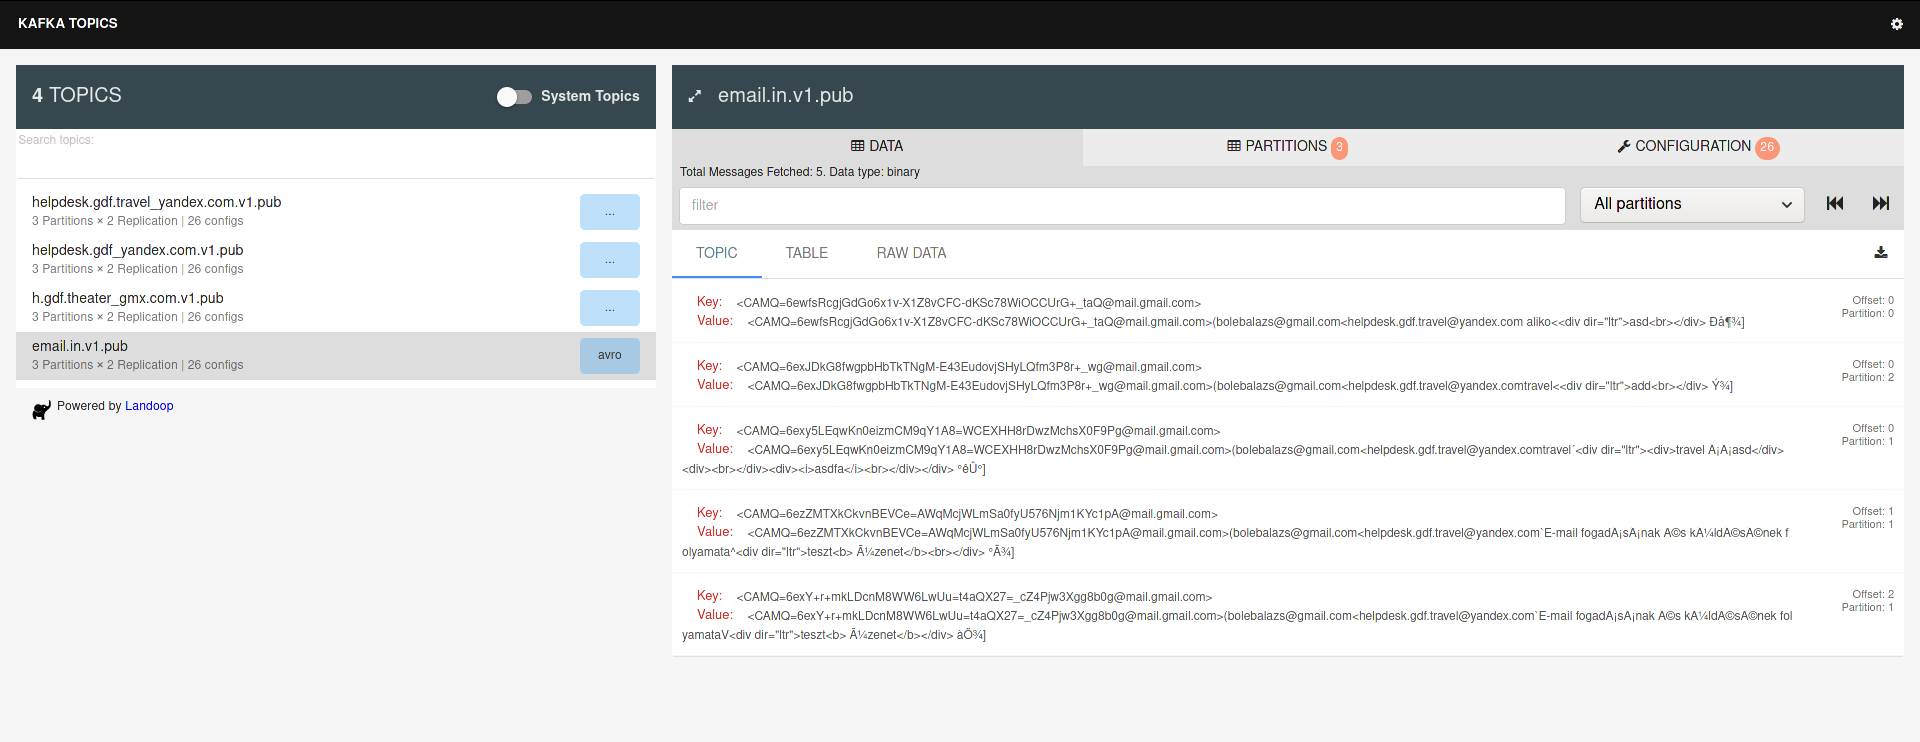
\includegraphics[width=0.9\textwidth]{Kafka_topic_ui.png}
	\caption[A Kafka Topics UI felülete]{A Kafka Topics UI eszközzel követhetőek a kafka \emph{topic}ok üzenetei, partíciói és beállításai}
	\label{fig:Kafka_Topics_UI}
	\floatfoot{Forrás: saját ábra}
\end{figure}


A helpdesk alakalmazás összesen hat \emph{topic}-ot használ:
\begin{description}
	\item[user.v1.pub] a Keycloak-ban regisztrált és karbantartott felhasználókat tartalmazza,
	
	\item[email.in.v1.pub] az összes beérkező  e-mailt tartalmazza,
	
	\item[helpdesk.gdf\textunderscore yandex.com.v1.pub] a  \href{mailto:helpdesk.gdf@yandex.com}{\nolinkurl{helpdesk.gdf@yandex.com}} címre küldött e-maileket tartalmazza,
	
	\item[helpdesk.gdf.travel\textunderscore yandex.com.v1.pub] a \href{mailto:helpdesk.gdf.travel@yandex.com}{\nolinkurl{helpdesk.gdf.travel@yandex.com}} címre küldött e-maileket tartalmazza,
	
	
	\item[h.gdf.theater\textunderscore gmx.com.v1.pub] a \href{mailto:h.gdf.theater@gmx.com}{\nolinkurl{h.gdf.theater@gmx.com}} címre küldött e-maileket tartalmazza,
	
	\item[\textunderscore schemas] a Schemaregistry ebben a \emph{topic}ban tárolja az alkalmazásban használt Avro schemákat.
\end{description}


Az alkalmazás három kafka brókert futtat egy clusterben, avagy számítógépfürtben. Továbbá minden üzleti funkcionalitást hordozó \emph{topic} --~a \textunderscore schemas-on kívül mindegyik~-- három partícióval és kettes replikációs faktorral lett létrehozva.
Így a kafka fürt egy bróker kiesése, vagy egy partíció sérülése esetén is működőképes marad.


\section{Eureka}
\Aref{sec:metrikak}. pontban említett szolgáltatások felderítésre az Eureka szervert használom. A helpdesk backend és az e-mail kliens az elindításuk után közvetlenül beregisztrálják magukat az Eureka szolgáltatásba.

Az Eureka szerveren keresztül megtekinthető és más szolgáltatások számára elérhető a példányok aktuális állapota és neve. Az oldal elérhető a \emph{Eureka service discovery} menüpont alatt~(\ref{fig:eureka}. ábra).


\begin{figure}[hbt] 
	\centering
	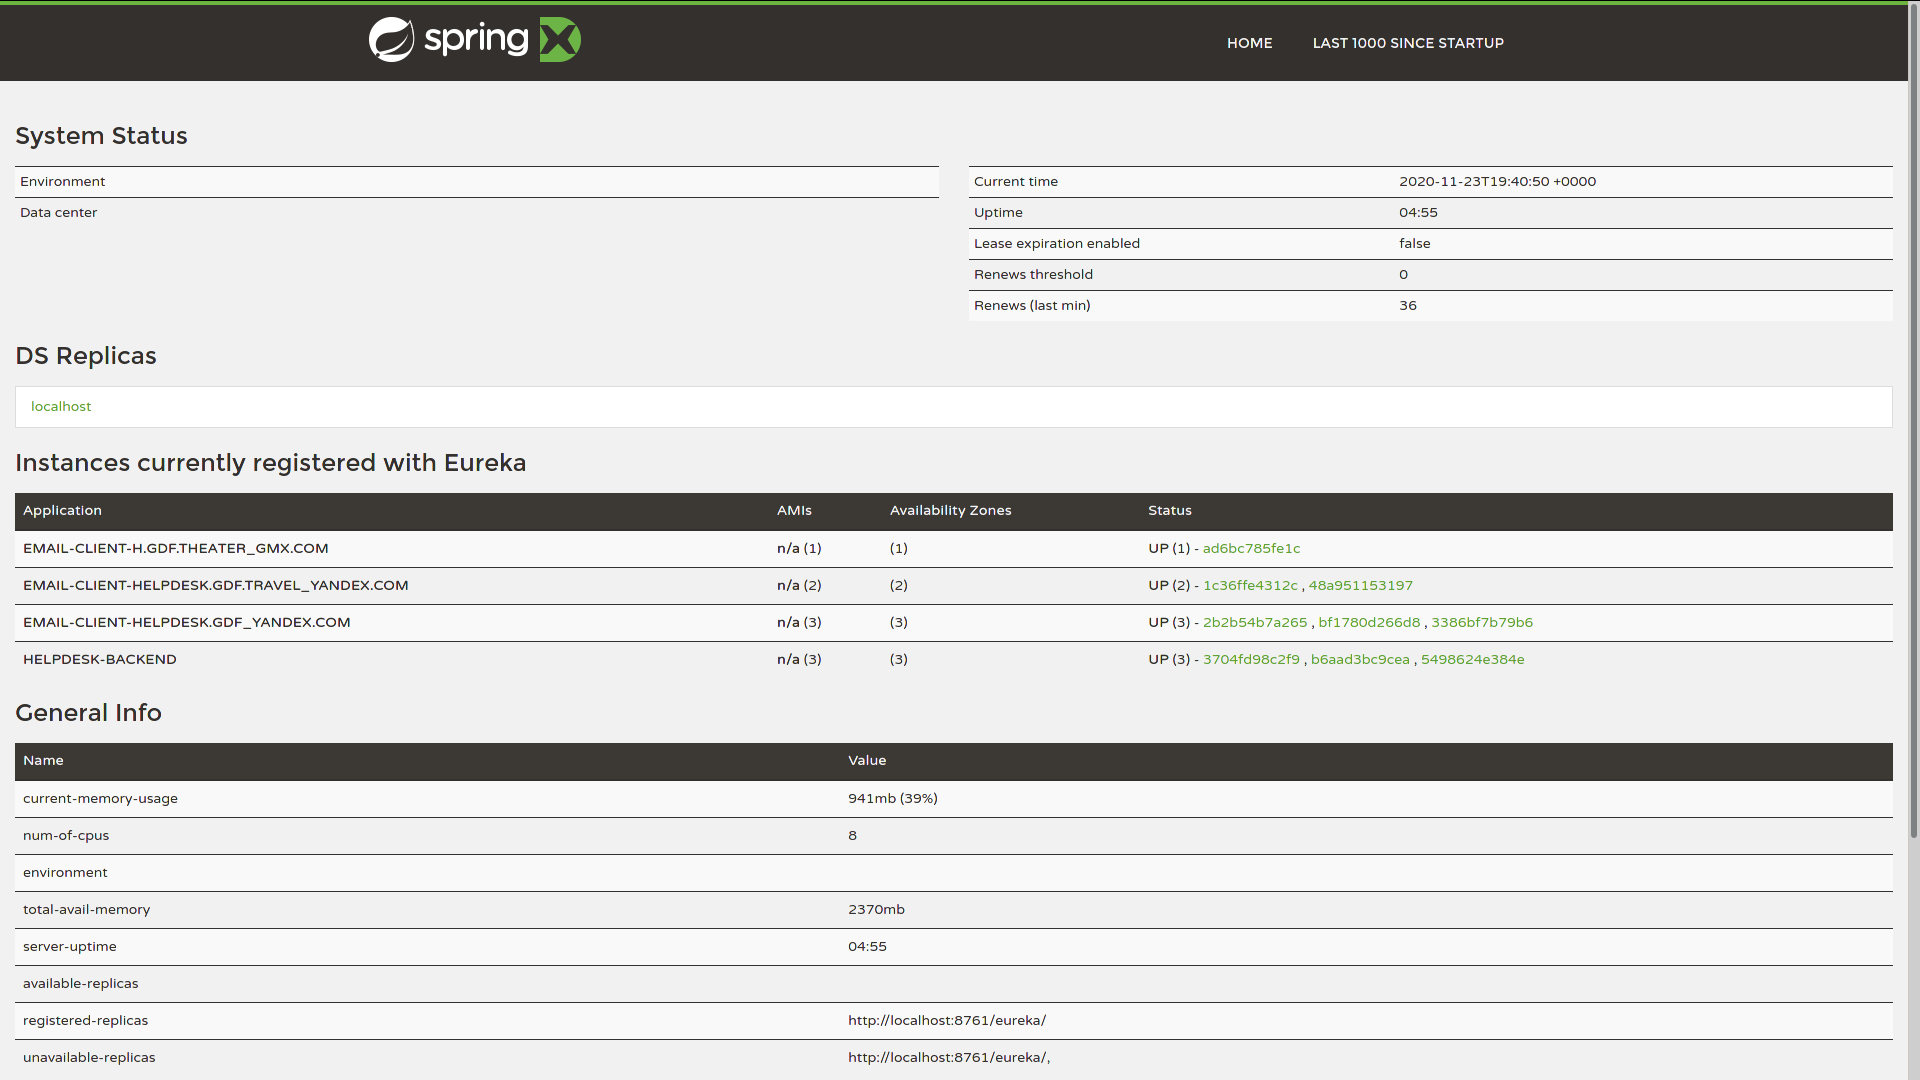
\includegraphics[width=0.85\textwidth]{eureka.png}
	\caption[Az Eureka service discovery felülete]{Az Eureka service discovery-n látható a mikroszerviz példányainak állapota és egyedi azonosítója}
	\label{fig:eureka}
	\floatfoot{Forrás: saját ábra}
\end{figure}

